% SC1005 --- Chapter 3: Combinational Logic (0->100)
\chapter{Combinational Logic: Adders, Multiplexers, Decoders}
\label{ch:combinational}

\begin{quote}
\emph{``Combinational means memoryless---output is a pure function of present inputs.''}
From gates we build arithmetic, selection, and routing---the data-path building blocks
every processor uses. No sequential knowledge assumed; we start from truth tables.
\end{quote}

\noindent\fbox{\parbox{\dimexpr\linewidth-2\fboxsep-2\fboxrule}{%
\textbf{From zero: gates $\to$ blocks.} We define combinational vs.\ sequential,
then derive each block from its truth table $\to$ Boolean expression $\to$ circuit.}}
\vspace{0.4em}

\section*{Learning Outcomes}
After this chapter you will be able to:
\begin{enumerate}[label=(L\arabic*)]
    \item distinguish combinational from sequential circuits;
    \item design half/full adders and ripple-carry adders from truth tables;
    \item use multiplexers as logic and routing elements;
    \item decode addresses with decoders and encode with priority encoders;
    \item analyse hazards and two-level vs.\ multi-level cost.
\end{enumerate}

% ============================================================
\section{Combinational Building Blocks}
\label{sec:comb-def}
A \emph{combinational} circuit has no memory: output at time $t$ depends only on inputs at $t$.
No feedback, no clock. Given $n$ inputs and $m$ outputs it realises a Boolean function
$f:\{0,1\}^n\to\{0,1\}^m$, fully specified by a truth table.

Design flow: (1) truth table, (2) SOP/POS or K-map to minimise (Ch.~\ref{ch:boolean}),
(3) map to available gates (NAND/NOR universality), (4) check delay and hazards.

\section{Adders: Half, Full, Ripple-Carry}
\label{sec:adders}
Adding is the first non-trivial combinational function. One column of binary addition
produces a sum bit and a carry.

\begin{definition}[Half and full adder]
\emph{Half adder} (HA): inputs $a,b$; outputs $S=a\oplus b$, $C_{\text{out}}=a\cdot b$
(adds two bits, no carry-in). \emph{Full adder} (FA): inputs $a,b,C_{\text{in}}$;
$S=a\oplus b\oplus C_{\text{in}}$, $C_{\text{out}}=ab+C_{\text{in}}(a\oplus b)$.
\end{definition}

\begin{figure}[h]
\centering
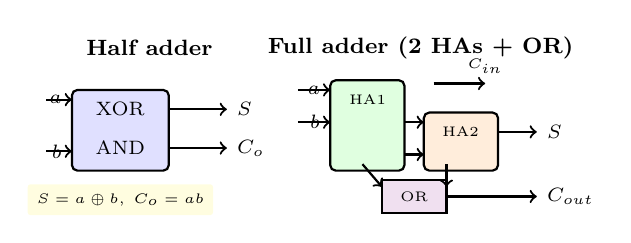
\begin{tikzpicture}[scale=0.82,every node/.style={font=\scriptsize}]
% Half adder
\node[font=\footnotesize\bfseries] at (1.6,2.0) {Half adder};
\draw[thick,fill=blue!12,rounded corners=2pt] (0.4,0.1) rectangle (1.9,1.35);
\node at (1.15,1.05) {XOR}; \node at (1.15,0.45) {AND};
\draw[->,thick] (0,1.2)--(0.4,1.2) node[left] {$a$};
\draw[->,thick] (0,0.4)--(0.4,0.4) node[left] {$b$};
\draw[->,thick] (1.9,1.05)--(2.8,1.05) node[right] {$S$};
\draw[->,thick] (1.9,0.45)--(2.8,0.45) node[right] {$C_o$};
\node[font=\tiny,fill=yellow!12,rounded corners=1pt] at (1.15,-0.35) {$S=a\oplus b,\;C_o=ab$};
% Full adder
\begin{scope}[xshift=4.2cm]
\node[font=\footnotesize\bfseries] at (1.6,2.0) {Full adder (2 HAs + OR)};
\draw[thick,fill=green!12,rounded corners=2pt] (0.2,0.1) rectangle (1.35,1.5);
\node[font=\tiny] at (0.78,1.2) {HA1};
\draw[thick,fill=orange!14,rounded corners=2pt] (1.65,0.1) rectangle (2.8,1.0);
\node[font=\tiny] at (2.22,0.7) {HA2};
\draw[->,thick] (-0.3,1.35)--(0.2,1.35) node[left] {$a$};
\draw[->,thick] (-0.3,0.85)--(0.2,0.85) node[left] {$b$};
\draw[->,thick] (1.8,1.45)--(2.6,1.45) node[above,font=\tiny] {$C_{\text{in}}$};
\draw[->,thick] (1.35,0.85)--(1.65,0.85);
\draw[->,thick] (1.35,0.35)--(1.65,0.35);
\draw[->,thick] (2.8,0.7)--(3.4,0.7) node[right] {$S$};
% OR for carry
\draw[thick,fill=violet!12] (1.0,-0.55) rectangle (2.0,-0.05);
\node[font=\tiny] at (1.5,-0.30) {OR};
\draw[->,thick] (0.7,0.2)--(1.0,-0.15); \draw[->,thick] (2.0,0.2)--(2.0,-0.15);
\draw[->,thick] (2.0,-0.30)--(3.4,-0.30) node[right] {$C_{\text{out}}$};
\end{scope}
\end{tikzpicture}
\caption{Left: half adder. Right: full adder built from two half adders plus OR for the carry. Coloured blocks match function.}
\label{fig:half-full-adder}
\end{figure}

Chaining FAs gives a \emph{ripple-carry adder} (RCA): $C_{\text{out}}$ of bit $i$ feeds
$C_{\text{in}}$ of bit $i+1$. Simple but carry ripples---delay $O(n)$ gate levels.
Faster adders (carry-lookahead, Ch.~\ref{ch:arithmetic}) compute carries in parallel.

\begin{figure}[h]
\centering
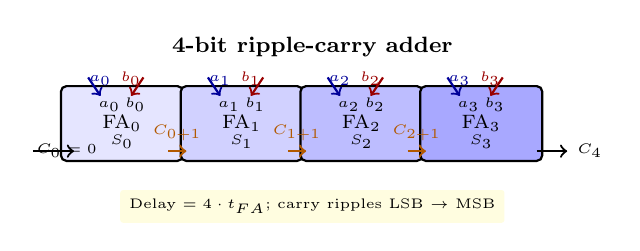
\begin{tikzpicture}[scale=0.78,every node/.style={font=\scriptsize}]
\node[font=\footnotesize\bfseries] at (4.0,1.85) {4-bit ripple-carry adder};
\foreach \i in {0,1,2,3} {
  \pgfmathsetmacro{\x}{\i*1.95}
  \node[draw,thick,fill=blue!\the\numexpr 10+\i*8\relax,minimum width=1.55cm,minimum height=0.95cm,rounded corners=2pt] at (\x+0.9,0.6) {FA$_{\i}$};
  \node[font=\tiny] at (\x+0.9,0.9) {$a_{\i}\;b_{\i}$};
  \node[font=\tiny] at (\x+0.9,0.3) {$S_{\i}$};
  \draw[->,thick,blue!60!black] (\x+0.35,1.35)--(\x+0.55,1.05) node[above,font=\tiny] {$a_{\i}$};
  \draw[->,thick,red!60!black] (\x+1.25,1.35)--(\x+1.05,1.05) node[above,font=\tiny] {$b_{\i}$};
}
\foreach \i in {0,1,2} {
  \pgfmathsetmacro{\x}{\i*1.95}
  \draw[->,thick,orange!70!black] (\x+1.65,0.15)--(\x+1.95,0.15) node[midway,above,font=\tiny] {$C_{\i+1}$};
}
\node[font=\tiny] at (0.0,0.15) {$C_0=0$} ; \draw[->,thick] (-0.55,0.15)--(0.12,0.15);
\draw[->,thick] (7.65,0.15)--(8.15,0.15) node[right,font=\tiny] {$C_4$};
\node[font=\tiny,fill=yellow!12,rounded corners=1pt] at (4.0,-0.75) {Delay $=4\cdot t_{\text{FA}}$; carry ripples LSB $\to$ MSB};
\end{tikzpicture}
\caption{Ripple-carry adder: four full adders chained. The carry path (orange) determines critical delay.}
\label{fig:ripple-adder}
\end{figure}

\section{Multiplexers and Demultiplexers}
\label{sec:mux}
A $2^n{\times}1$ \emph{multiplexer} (MUX) selects one of $2^n$ data inputs via $n$ select lines;
a \emph{demultiplexer} does the reverse. A MUX is a universal logic block: any $n$-variable
function can be realised by wiring its truth table to data inputs and variables to selects.

\begin{figure}[h]
\centering
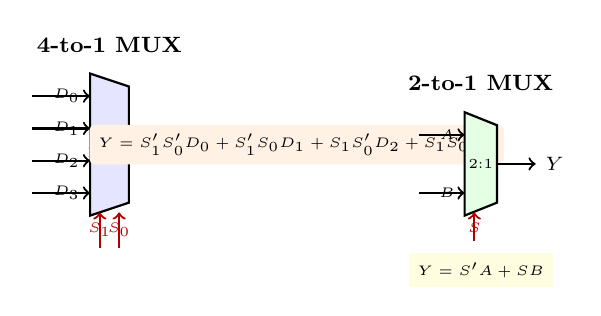
\begin{tikzpicture}[scale=0.82,every node/.style={font=\scriptsize}]
% 4:1 MUX
\draw[thick,fill=blue!10] (0,0) -- (0,2.2) -- (0.6,2.0) -- (0.6,0.2) -- cycle;
\foreach \y/\lbl in {1.85/$D_0$,1.35/$D_1$,0.85/$D_2$,0.35/$D_3$} \draw[->,thick] (-0.9,\y)--(0,\y) node[left,font=\tiny] {\lbl};
\draw[->,thick,red!70!black] (0.15,-0.5)--(0.15,0.05) node[below,font=\tiny] {$S_1$};
\draw[->,thick,red!70!black] (0.45,-0.5)--(0.45,0.05) node[below,font=\tiny] {$S_0$};
\draw[->,thick] (0.6,1.1)--(1.4,1.1) node[right] {$Y$};
\node[font=\tiny,align=center] at (0.3,1.1) {4:1\\MUX};
\node[font=\footnotesize\bfseries] at (0.3,2.65) {4-to-1 MUX};
% Equation
\node[font=\tiny,fill=orange!10,rounded corners=2pt] at (3.2,1.1) {$Y=S_1'S_0'D_0+S_1'S_0D_1+S_1S_0'D_2+S_1S_0D_3$};
% 2:1 MUX as gate
\begin{scope}[xshift=5.8cm]
\draw[thick,fill=green!10] (0,0) -- (0,1.6) -- (0.5,1.4) -- (0.5,0.2) -- cycle;
\draw[->,thick] (-0.7,1.25)--(0,1.25) node[left,font=\tiny] {$A$};
\draw[->,thick] (-0.7,0.35)--(0,0.35) node[left,font=\tiny] {$B$};
\draw[->,thick,red!70!black] (0.15,-0.4)--(0.15,0.05) node[below,font=\tiny] {$S$};
\draw[->,thick] (0.5,0.8)--(1.1,0.8) node[right] {$Y$};
\node[font=\tiny] at (0.25,0.8) {2:1};
\node[font=\tiny,fill=yellow!12] at (0.25,-0.85) {$Y=S'A+SB$};
\node[font=\footnotesize\bfseries] at (0.25,2.05) {2-to-1 MUX};
\end{scope}
\end{tikzpicture}
\caption{Multiplexers: $4{:}1$ selects one of four data lines; $2{:}1$ realises $Y=S'A+SB$. Select lines in red.}
\label{fig:mux}
\end{figure}

\section{Decoders, Encoders, and Tri-State}
A $n$-to-$2^n$ \emph{decoder} asserts exactly one of $2^n$ outputs for each input code
(address decoding). A \emph{priority encoder} reverses this, reporting the highest-priority active input.
\emph{Tri-state} buffers allow bus sharing: output is $0$, $1$, or high-impedance $Z$ (disconnected).

Hazards: combinational glitches when inputs change (static hazard: momentary $0$ or $1$ spike).
K-map grouping with overlapping prime implicants or adding hazard covers fixes it for two-level logic.


\section{Comparators, Code Converters, and Hierarchical Design}
Beyond adders and MUXes, two more combinational staples appear everywhere.
A \emph{magnitude comparator} reports $A>B$, $A=B$, $A<B$ via subtraction without storing the difference:
$A-B$ sign and zero flags give the answer. A \emph{code converter} (e.g.\ binary to Gray or BCD to 7-segment)
is simply a truth table mapped to SOP with don't-cares for unused codes.

Hierarchical design builds large blocks from small: an 8-bit RCA from two 4-bit RCAs, a 16-to-1 MUX from five 4-to-1 MUXes,
a 5-to-32 decoder from 2-to-4 plus 3-to-8 decoders with enables. Enables ($\overline{EN}$) are the glue---inactive blocks
output $0$ or $Z$, so only the selected block drives the bus.
\begin{example}[7-segment decoder]
Hex digit $h_3h_2h_1h_0$ drives segments $a$--$g$. Row $h=0000$ lights $a,b,c,d,e,f$ but not $g$ (displays `0').
K-maps for each segment share product terms---multi-output minimization saves gates versus per-output solo maps.
\end{example}

% ============================================================

% ============================================================
\section{Chapter Notes}
Claude Shannon's switching algebra (1938) first mapped Boolean functions to relay circuits.
MUX-based design became popular with MSI chips (74151, 74138) in the 1970s TTL era.

% ============================================================
\section{Timing and Hazards in Combinational Logic}
Gate delay matters. The \emph{critical path} is the longest input-to-output chain; its delay sets the minimum clock period
for the surrounding sequential system. A \emph{static hazard} is a momentary glitch when one input changes but the output
should stay constant---caused by unequal path delays reconverging (e.g.\ $F=x\bar x$ momentarily $1$ during transition).
A \emph{dynamic hazard} toggles multiple times before settling.

K-maps naturally reveal static hazards: any adjacent $1$s not covered by a common implicant is a potential glitch when
crossing between them. Adding the \emph{consensus} implicant that bridges the adjacency removes the hazard (at the cost of one extra term).
Modern synthesis with multi-level logic may still introduce hazards---hazard-free design or registered outputs (Ch.~\ref{ch:sequential}) solves it.

% ============================================================

\paragraph{Bus and tri-state.} Multiple combinational blocks sharing a bus use \emph{tri-state} buffers ($0/1/Z$).
Only one driver is enabled at a time; the bus is a wired-OR of tri-states. Modern CMOS prefers MUX-based buses internally
(lower contention risk) with tri-states reserved for off-chip or bidirectional pins. Forgetting the enable decode is a classic
lab bug---two drivers fighting draws large shoot-through current.

\section{Exercises}
\label{sec:ch03-exercises}
\begin{enumerate}[label=E3.\arabic*, leftmargin=*, itemsep=0.8em]
    \item \textbf{Full adder proof.} From the truth table derive $S$ and $C_{\text{out}}$ expressions, then show $C_{\text{out}}=ab+C_{\text{in}}(a\oplus b)=ab+aC_{\text{in}}+bC_{\text{in}}$.
    \item \textbf{Ripple delay.} A FA has delay $2$ gate levels for $S$ and $1$ for $C_{\text{out}}$. What is worst-case delay of an 8-bit RCA? Where is the critical path?
    \item \textbf{MUX as logic.} Realise $F(x,y,z)=\sum m(1,2,5,6)$ using (a) an 8:1 MUX, (b) a 4:1 MUX with $x$ as data, (c) only 2:1 MUXes.
    \item \textbf{Decoder expansion.} Build a 4-to-16 decoder from 2-to-4 decoders and gates. How many 2-to-4 blocks are needed? Draw the enable wiring.
    \item \textbf{Hazard.} $F=x y + x' z$ glitches when $y=z=1$ and $x$ toggles. Show the K-map, identify the hazard, and add the consensus term $y z$ to remove it.
\end{enumerate}
% End of Chapter 3
